Clase: 25/11/2022


\begin{teorema}[5I]
    Si $F$ y $F'$ son campos, $\tau:F\to F'$ es un isomorfismo, $p(x)\in F[x]$ es irreducible sobre $F$ y $v$ es una raíz de $p(x)$, entonces existe $\sigma:F(v)\to F'(w)$, isomorfismo, donde $w$ es una raíz de $p'(t)=\tau^*(p(x))$, y este isomorfismo $\sigma$ puede elegirse tal que:
    \begin{enumerate}
        \item $\sigma(v)=w$
        \item $\sigma(\alpha)=\tau(\alpha)=\alpha',\forall \alpha \in F$. Es decir, $\sigma$ deja fijos (salvo el isomorfismo) a los elementos de $F$
    \end{enumerate}
    \begin{dem}
        Considere $M=\{f(x)\in F[x]:f(v)=0\}$. Si $f_1(x),f_2(x)\in M\implies f_1(v)-f_2(v)=0-0=0\implies f_1(x)-f_2(x)\in M\implies$ por el corolario al lema 2.3 $(M,+)$ es subgrupo de $(F[x], +)$. Si $g(x)\in F[x]$ y $f(x)\in M\implies g(v)f(v)=g(v)=0=0\implies g(x)f(x)\in M\implies M$ es un ideal de $F[x]$.Además, $p(v)=0\implies p(x)\in M\implies (p(x))\subseteq M$.
        Como existen polinomios en $F[x]$, no satisfechos por $v\implies M\subset F[x]$, no satisfechos por $v\implies M\subset F[x]$. Pero, siendo $p(x)$ irreducible sobre $F$, por el lema 3.22, $(p(x))$ es un ideal maximal en $F[x]\implies M=(p(x))$. Considérese el homomorfismo $\psi:F[x]\to F[v]\ni \psi(f(x))=f(v)$ empleando los argumentos de la prueba de los teoremas 5.B.C.G, $\psi$ es un homomorfismo $\ni K_\psi =M=(p(x))$ y existe $\psi^* F[x]/(p(x))\to F(v)\ni \psi^*(f(x)+[p(x)])=f(v)$, isomorfismo.
        
        
        $F[x]/(p(x))\approx F(v)$ 
        \begin{figure}[H]
            \centering
            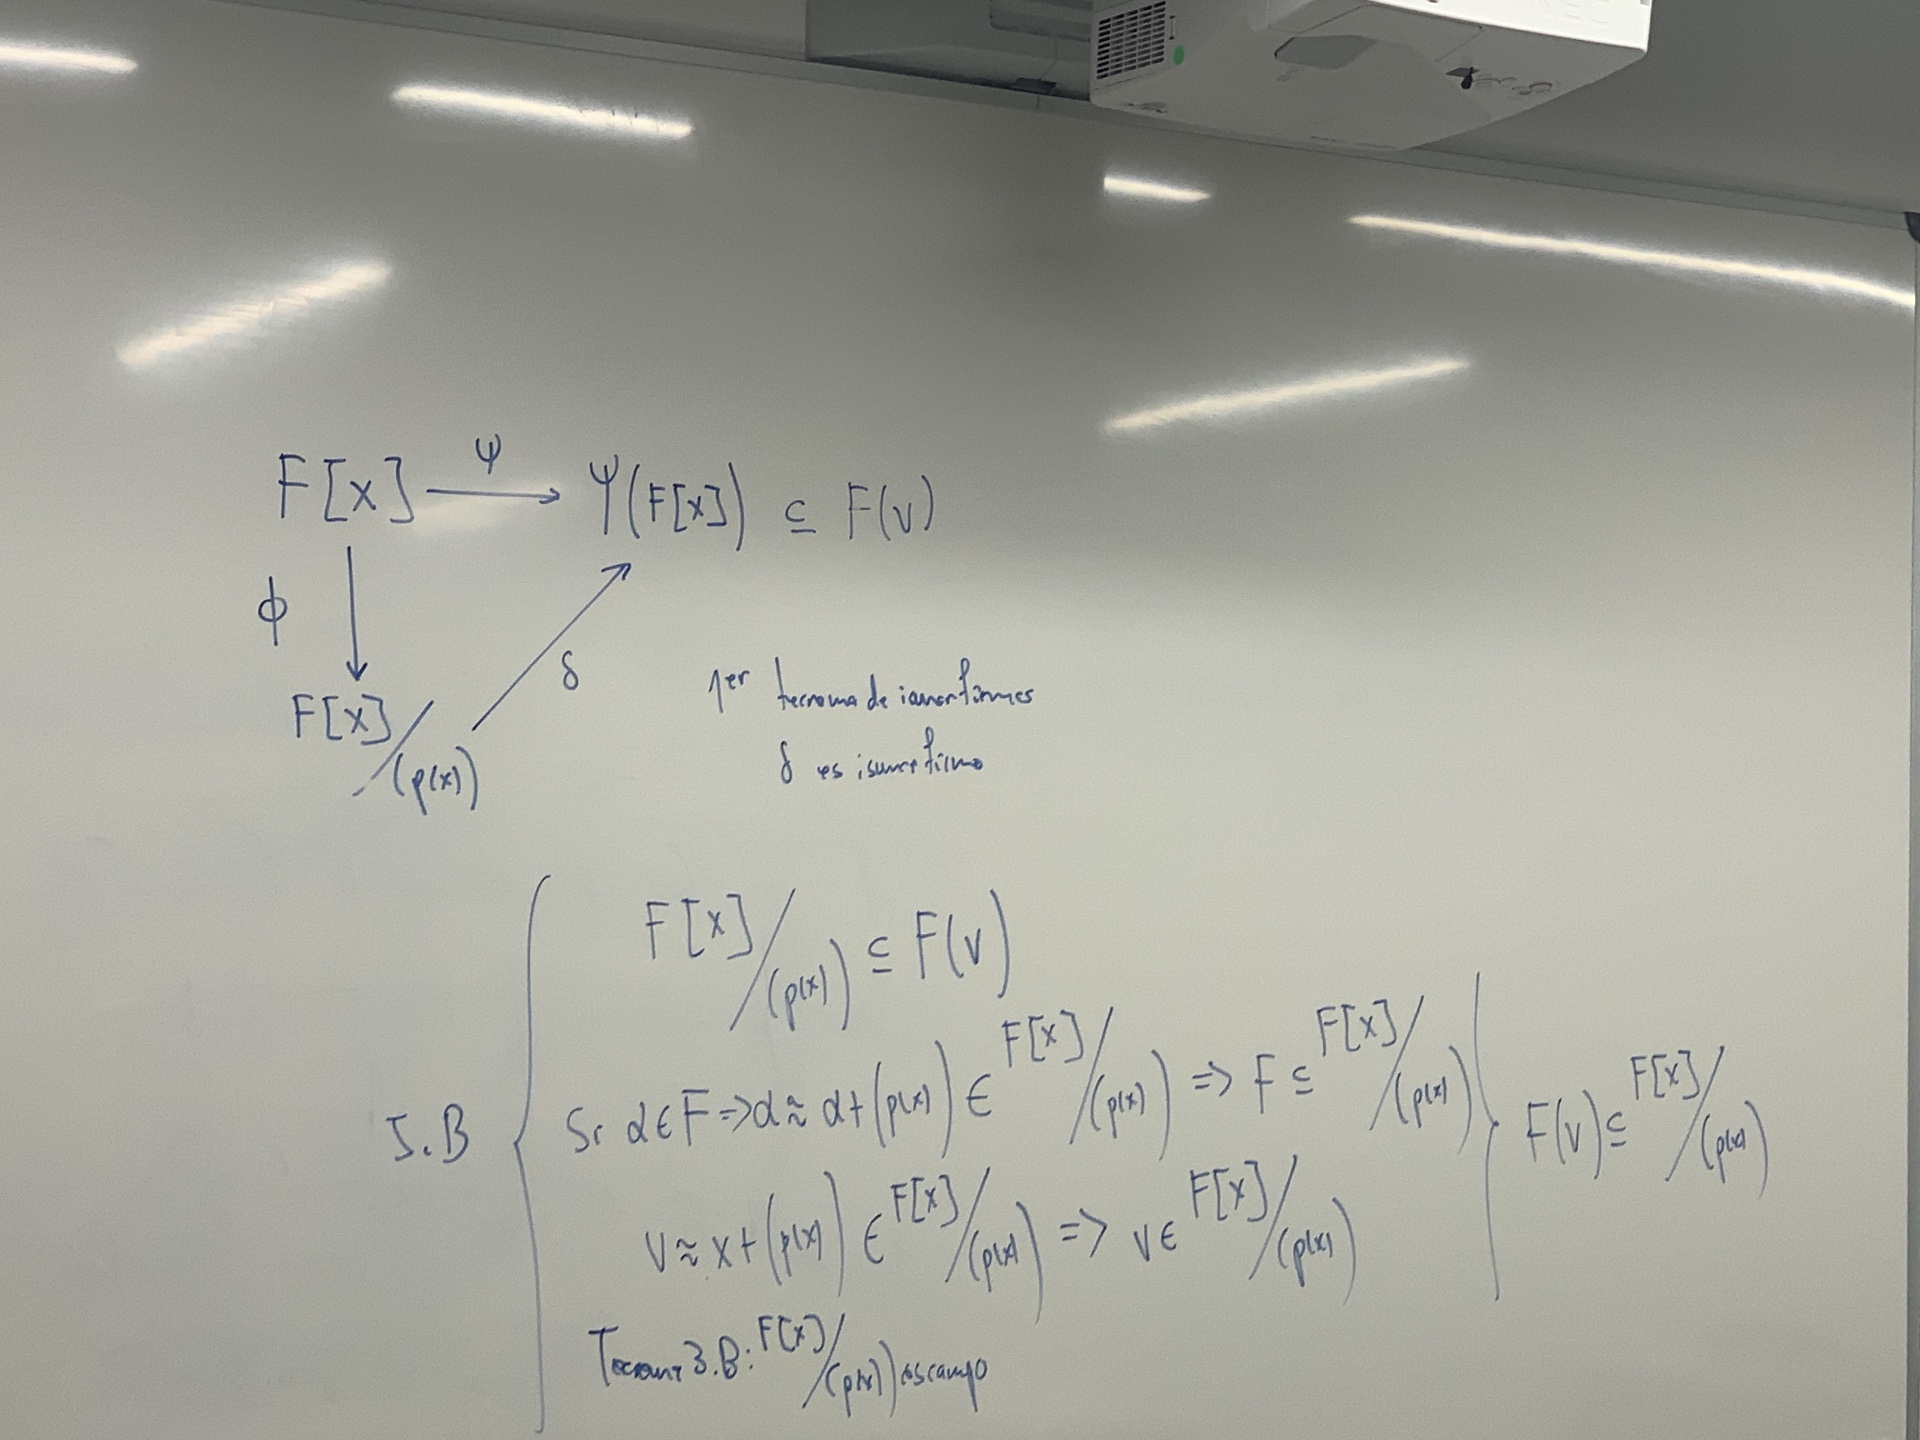
\includegraphics[scale=0.2]{imagenes/25.1.jpeg}
        \end{figure}
        Como $p(x)$ es irreducible en $F[x]$ y por el lema 5.3 $\tau^*:F[x]\to F'[t]$ es un isomorfismo entonces $\tau^*(p(x))=p'(t)$ es irreducible en $F'[t]$. Entonces replicando los argumentos ya usados, existe $\theta^*: F'[t]/(p'(t))\to F(w)\ni \theta^*(f'(t)+[p'(t)])=f'(w)$, isomorfismo. Además, por el lema 5.4, $\tau^{**}:F[x]/(p(x))\to F'[t]/(p'(t))\ni \tau^{**}(f(x)+[p(x)])=f'(t)+(p'(t))$ es un isomorfismo de campos $\ni$ si $\alpha\in F\implies \tau^{**}(\alpha)\approx \tau^{**}(\alpha+(p(x)))=\tau(\alpha)+(p'(t))=\alpha' +(p'(t))\approx \alpha'$ y $\tau^{**}(x+(p(x)))=\tau^{*}(x)+(p'(t))=t+(p'(t))$. Considérese el siguiente diagrama: 
        \begin{figure}[H]
            \centering
            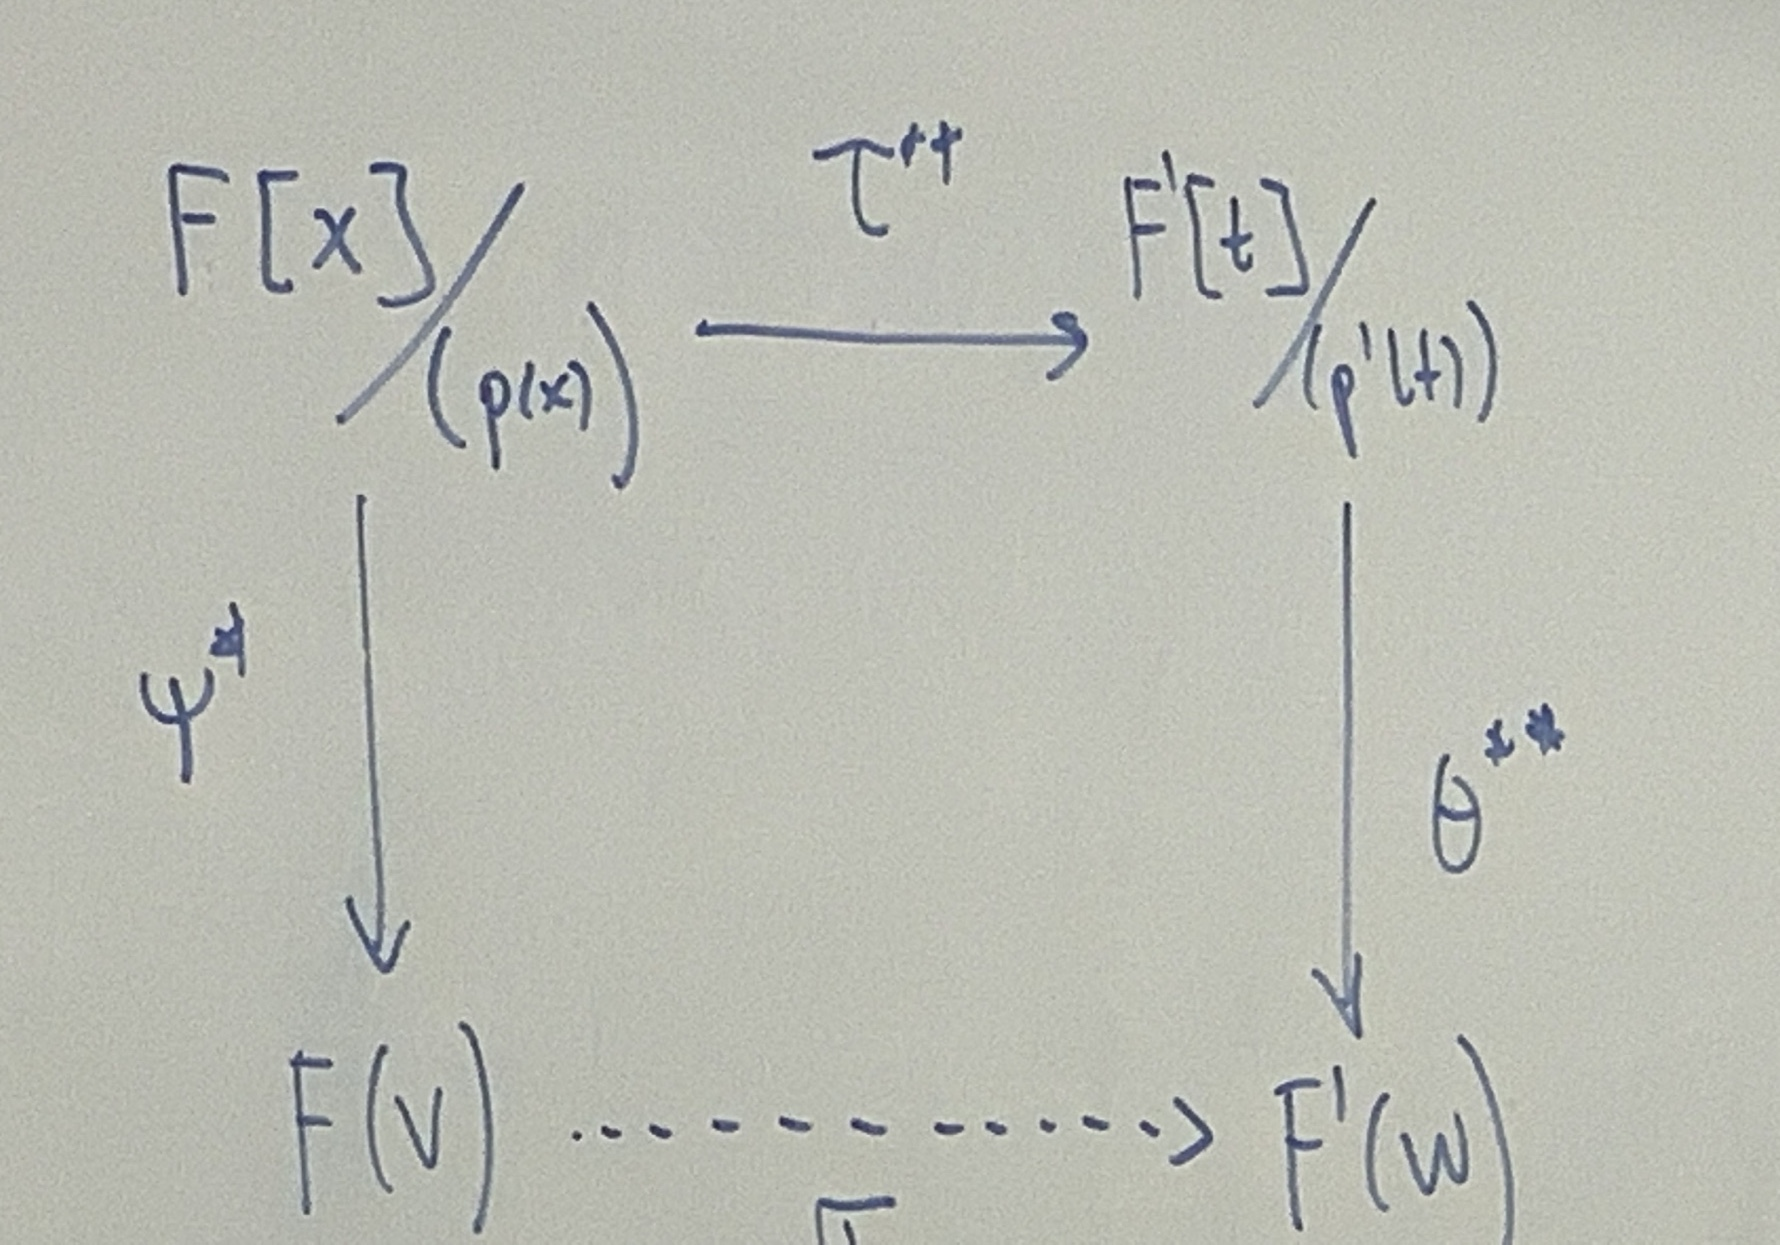
\includegraphics[scale=0.15]{imagenes/25.2.jpeg}
        \end{figure}
    \end{dem}
    \begin{cajita}
        Si $F=F'$ (automorfismo), y donde $\sigma:F(v)\to F(w)$ y más precisamente $\sigma|_F = I_F$
    \end{cajita}
    y la función $\sigma=(\psi^*)^{-1}\tau^{**}\theta^*: F(v)\to F'(w)$, un isomorfismo, por ser la composición de isomorfismos. Nótese que $\sigma(v)=(\psi^{*})^{-1}\tau^{**}\theta^{**}(v)=\theta^{**}(\tau^{**}(\psi^{*-1}(v)))=_{5B}=\theta^{**}(\theta^{**}(x+(p(x))))= \theta^{**}(t+(p'(t)))=w$ y si $\alpha\in F\implies \sigma(\alpha)=\psi^{*-1}\tau^{**}\theta^{**}(\alpha)=\theta^{**}(\theta^{**}(\psi^{*-1}(\alpha)))=\theta^{**}(\tau^{**}(\alpha +p(w)))=\theta^{**}(\tau^{*}(\alpha)+(p'(t)))=_{5.3}=\theta^{**}(\tau(\alpha)+p'(t))=\theta^{**}(\alpha'+(p'(t)))=\alpha'$.
\end{teorema}

\begin{corolario}
    Si $F$ es un campo, $p(x)\in F[x]$ es irreducible sobre $F$ y $a,b$ son raíces de $p(x)$ entonces existe $\sigma: F(a)\to F(b)$, isomorfismo, tal que $\sigma(a)=b$ y $\sigma(\alpha)=\alpha$, $\forall \alpha \in F$.
    \begin{dem}
        Aplíquese el teorema 5I al caso especial $F=F'$ y $\tau =I_F$.
    \end{dem}
\end{corolario}

